\section{NMT}\label{Appendix:A}
Esta es una entidad de la capa de aplicación que permite el correcto
funcionamiento de la red. Esta entidad tiene los servicios necesarios para que
cada nodo tenga un conocimiento de todos los nodos conectados en la red. Esto
permite el armado de una tabla de nodos, que es mantenida en todo los
nodos. Esta entidad exige la existencia de un nodo monitor, que es el encargado
de monitorear y configurar la red. Luego, una vez en funcionamiento este nodo
monitor no será vital para la red. En el NMT se deben implementar los
algoritmos de ruteo. El entorno NMT se puede observar en la Figura \ref{fig:NMT}

\begin{figure}[h!]
 \centering
 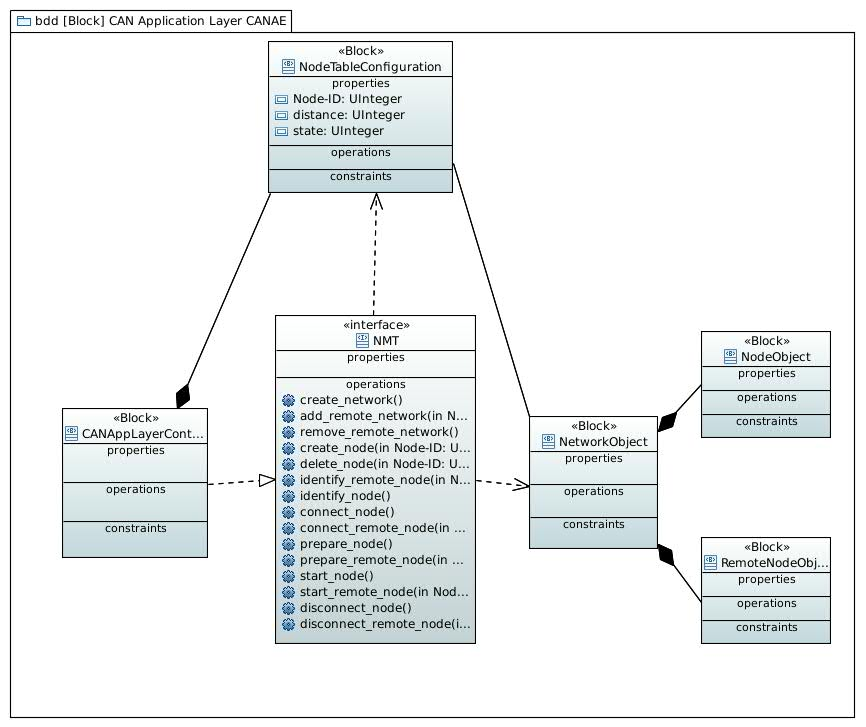
\includegraphics[scale=0.4]{images/Secciones/AppendixA/NMT.JPG}
  \caption{Definición de la entidad NMT}
\label{fig:NMT}
\end{figure} 

Por medio de este servicio es posible conocer el estado de la red CAN. Los
mensajes de NMT CAN son envíados con máxima prioridad. 
\subsection{Objectos NMT}
El Network Management utiliza tres objetos diferentes para modelar una red CAN.
\begin{itemize}
 \item \textbf{Network Object}: Representa todos los modulos conectados en la
  red CAN. El objeto de red existe en todos los nodos.
 \item \textbf{Remote Node Object}: Cada nodo conectado a la red CAN tiene
   representado todos los demás nodos.    
 \item \textbf{Node Object}: Cada nodo que es gestionado por el servicio NMT
   está representado por un node object. Este objeto se encuentra modelado en
   cada uno de los nodos.    
 \end{itemize}
Cada nodo y su objeto (remoto y local) es unívocamente identificado en la red
por su NMT Address. Esta dirección no se puede cambiar. Esto significa que por
cada nodo existe un objeto nodo y un objeto nodo remoto con el mismo NMT
Address, replicada en todos los nodos de la red. 

\subsection{Servicios NMT}
La entidad NMT ofrece los siguientes servicios:
\subsubsection{Module Control Service}
EL NMT monitor incializa los nodos NMT que forman parte de la red CAN
distribuida, a través de este servicio se asegura que todos los nodos se
encuentran configurados y funcionando correctamente.
\subsubsection{Error Control Services}
Através de este servicio, el NMT detecta fallas en la red CAN, ya sea fallas
producidas en la capa de enlace de datos (fallas locales) y/o fallas
producidos en otros nodos.
\subsubsection{Configuration Control Services}
Através de este servicio se realiza la configuarción de la red.

\subsubsection{Servicios a implementar}
La funciones típicas que se deben implementar en el NMT son los siguientes:
\begin{itemize}
\item Boolean create\_network()
\item Boolean create\_remote\_network() 
\item Boolean remove\_remote\_network()
\item Boolean create\_node(UInteger Node-ID, UInteger address, String description)
  \begin{itemize}
  \item \textbf{UInteger Node-ID}: ID del nodo a crear.
  \item \textbf{UInteger address}: Dirección del nodo creado. UInteger entre [0,255]
  \item \textbf{String description}: Descripción del nodo.
  \end{itemize}
\item Boolean delete\_node(UInteger Node-ID)
  \begin{itemize}
   \item \textbf{UInteger Node-ID}: Dirección del nodo a eliminar. UInteger entre [0,255]
  \end{itemize}
    
\item UInteger identify\_remote\_node(UInteger Node-ID)
  \begin{itemize}
  \item \textbf{UInteger Node-ID}: Dirección del nodo a idetenficar
  \end{itemize}

\item UInteger identify\_node()
  
\item Boolean connect\_node()
  
\item Boolean connect\_remote\_node(UInteger Node-ID)
  \begin{itemize}
    \item \textbf{UInteger Node-ID}: ID del nodo remoto a conectar.
  \end{itemize}

\item Boolean prepare\_node()
\item Boolean prepare\_remote\_node(UInteger Node-ID)
  \begin{itemize}
   \item \textbf{UInteger Node-ID}: ID del nodo a pasar a modo preparado
  \end{itemize}
\item Boolean start\_node()
\item Boolean start\_remote\_node(UInteger Node-ID)
  \begin{itemize}
    \item \textbf{UIntenger Node-ID}: ID del nodo que comenzará a participar en la red.
   \end{itemize}
\item Boolean disconnect\_node()
\item Boolean disconnect\_remote\_node(UInteger Node-ID)
  \begin{itemize}
    \item \textbf{UInteger Node-ID}: ID del nodo a desconectar.
  \end{itemize}
\end{itemize}

\subsection{Protocolos NMT}
\subsubsection{Crear red CANae}
Para conectar correctamente la red CANae se debe respetar el protocolo NMT para crear la red.
En primer lugar el nodo monitor debe enviar el mensaje \textit{create\_remote\_network()}
para avisar a todos los nodos que deben crear sus propias instancias de
\textit{NetworkObject} a través de \textit{create\_network()}. Automáticamente, los nodos deben crear una propia instancia del nodo mediante
\textit{create\_node()}. Luego el nodo monitor envía el mensaje de
\textit{prepare\_remote\_node()} para prepara todos los nodos a conectarse a la red CANae.
Luego el nodo monitor envía la señal de \textit{connect\_remote\_node(UInteger Node-ID)} con
la dirección de todos los nodos que figuran en su \textit{NodeTableConfiguration}
preprogramada.
Luego cada nodo, correctamente preparado, se conecta a la red a través de
\textit{connect\_node()}.

Este protocolo puede ser observado en la Figura \ref{fig:ProtocolNMTConnectNet}
\begin{figure}[h!]
 \centering
 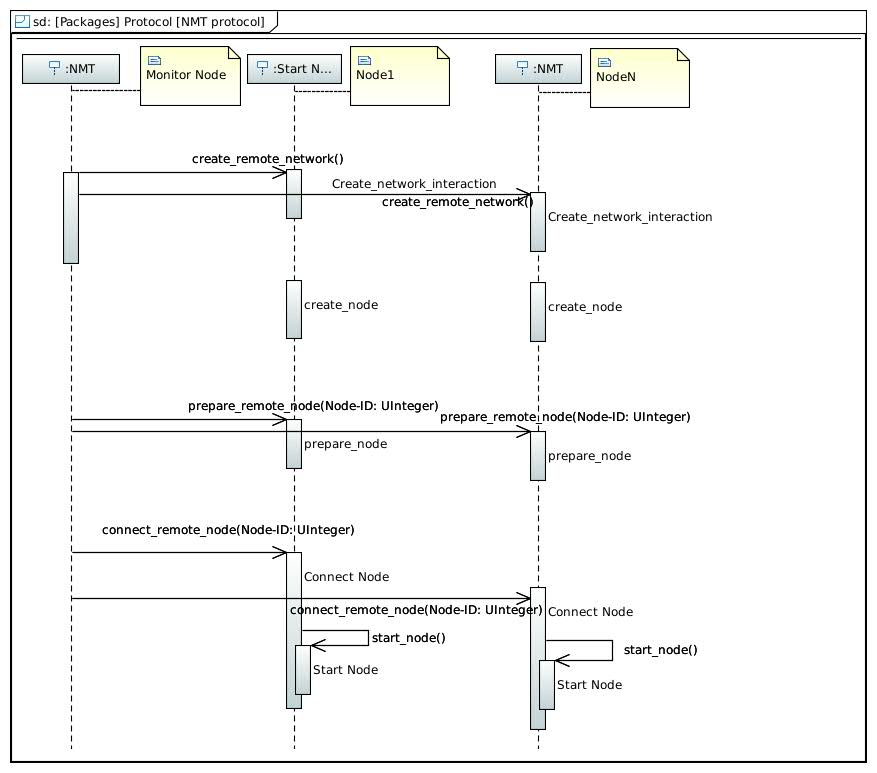
\includegraphics[scale=0.4]{images/Secciones/AppendixA/Protocol_NMT.JPG}
  \caption{Protocolo NMT}
  \label{fig:ProtocolNMTConnectNet}
\end{figure} 

\subsubsection{Crear Red}\label{NMT:crear_red}
Para lograr la correcta conexión de los nodos a la red, estos deben
configurarse. Cuando se alimenta la red, los nodos deben iniciar en estado de
\textit{escucha} esperando la orden del nodo monitor de crear la red mediante
\textit{create\_remote\_network()}. Esta se envía en broadcast a todos los nodos
conectados. Cuando el controlador de la capa de aplicaciónr recibe el mensaje
através del servicio NMT, este manda un mensaje al gesto del nodo interno, el
cual crea la \textit{tabla de configuración del nodo} y acutizaliza con la
información necesaria.

\begin{figure}[h!]
 \centering
 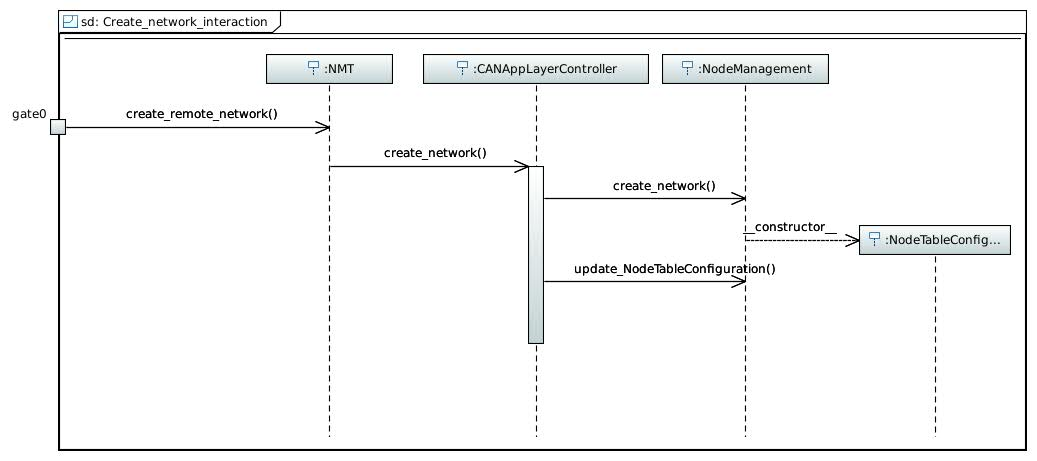
\includegraphics[scale=0.4]{images/Secciones/AppendixA/Create_Network.JPG}
  \caption{Crear Red}
  \label{fig:ProtocolNMTConnectNet}
\end{figure} 

\subsubsection{Crear Objecto Red, Objeto Nodo y Objeto Nodo Remoto}
Antes de comenzar a funcionar la red, cada nodo debe crear un objeto de red
exigidos por el protocolo NMT. Una vez que el proceso Crear Red termina,
el Gestor de la capa de Aplicación envía un mensaje \textit{create\_node()}
al Gestor del Nodo. El Gestor de Nodo crea un \textit{Network Object}. Este a su
vez crea un \textit{Node Object} y un \textit{Remote Node Object}. Estos objetos
pertenecen a la entidad NMT.

\begin{figure}[h!]
 \centering
 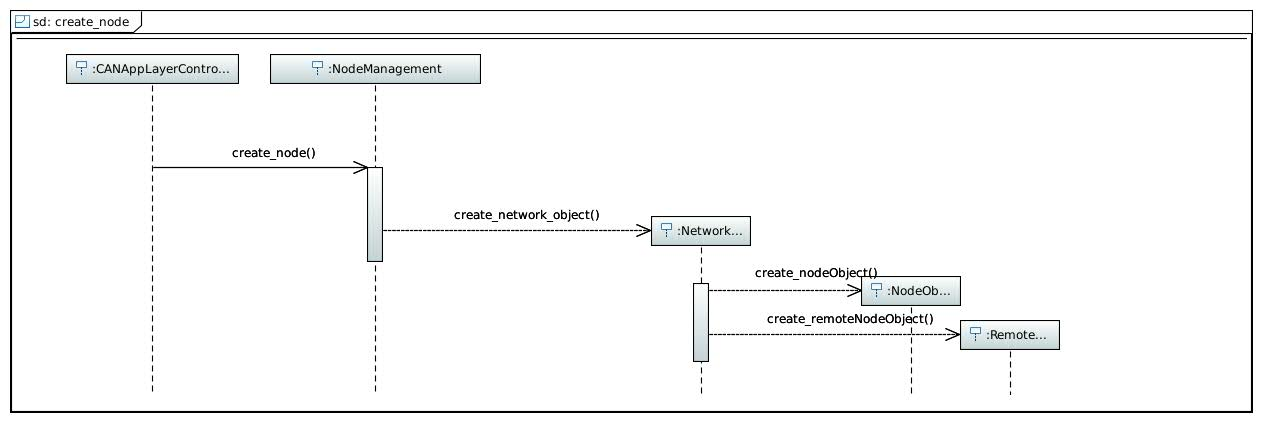
\includegraphics[scale=0.4]{images/Secciones/AppendixA/create_node.JPG}
  \caption{Crear Objecto Red, Objeto Nodo y Objeto Nodo Remoto}
  \label{fig:ProtocolNMTConnectNet}
\end{figure}






























































































































































































































